\frame{
\frametitle{Experiments}
\begin{textblock*}{90mm}[0,0](-8mm,-2mm)
	\textcolor{myred}{\textbf{Turbulent generators}}
\end{textblock*}

\begin{textblock*}{125mm}[0,0](-8mm,2mm)
{\small
\begin{itemize}
\item Wind tunnels:\vspace{-6pt}
	\begin{itemize}
		\item passive or active grids 
		\item \textit{good homogeneity and isotropy}
		\item \textit{strong mean flow}
	\end{itemize}
\item Turbulent boxes:\vspace{-6pt}
	\begin{itemize}
	\item von K\'arm\'an	
	\item polyhedra with fans / motors
	\item oscillating grids
	\item synthetic jets
	\item \textit{vanishing mean low}
	\item \textit{recirculation problem}
	\end{itemize}
\item In situ measurements
\end{itemize}
}
\vspace{4pt}
\only<1>
\small{\textbf{	\textcolor{myred}{Trade off:}}}\vspace{-4pt}
\begin{itemize}
	\item Homogenity and sotropy \vspace{-6pt}
	\item Turbulence level $R_{\lambda}$ \vspace{-6pt}
\end{itemize}
\end{textblock*}
%
%

\begin{textblock*}{80mm}[0,0](65mm,28mm)
	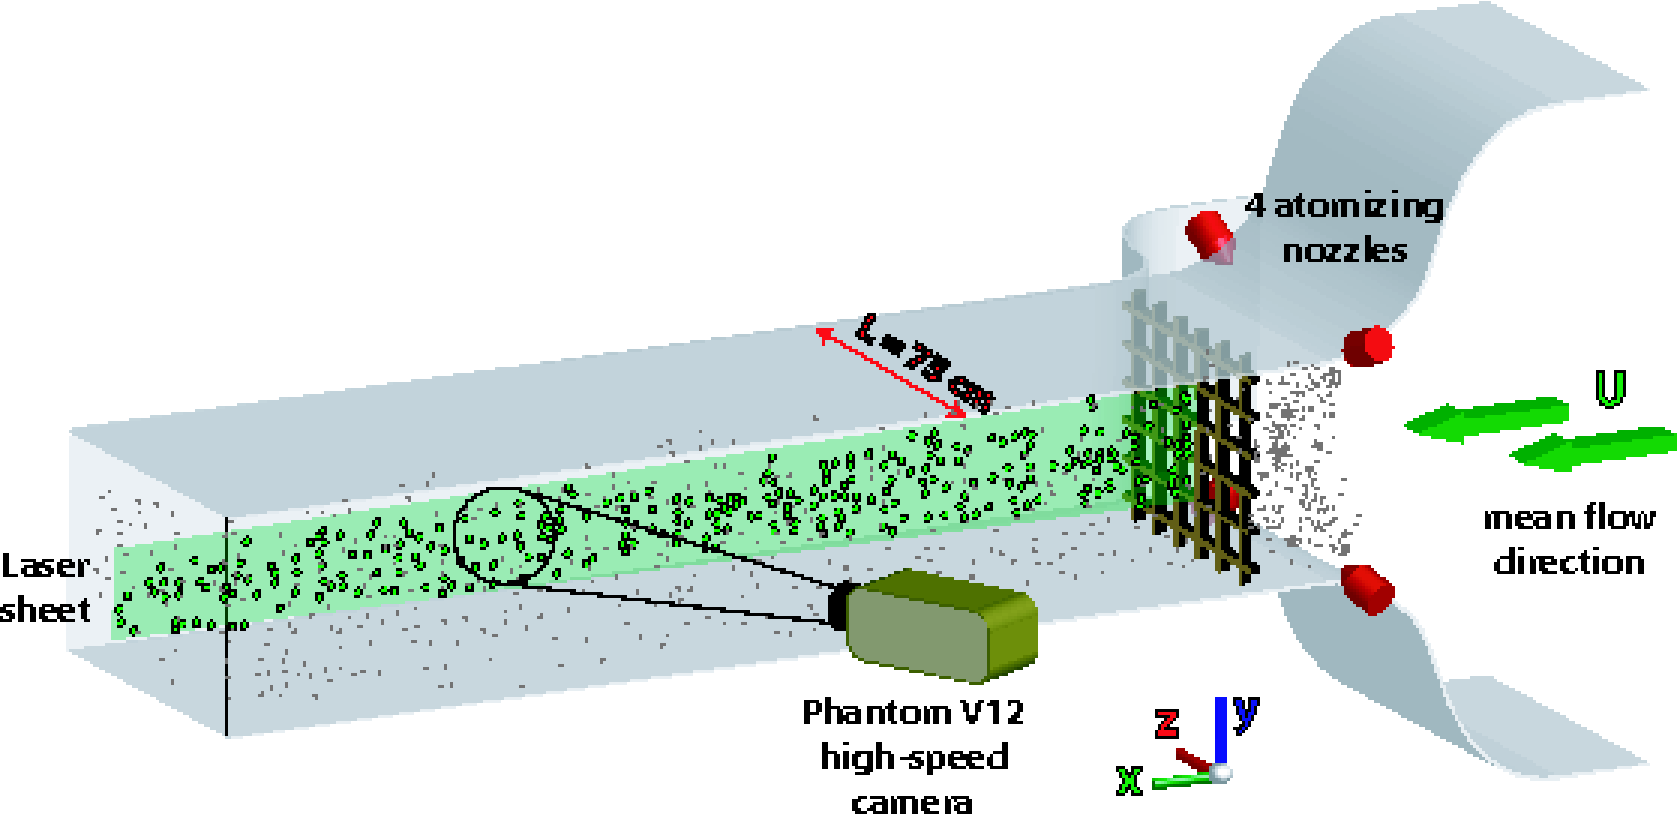
\includegraphics[height = 24mm]{experimentRain.pdf}\\
	\vspace{-12pt}
	{\flushright {\tiny Wind tunnel: Monchaux et al, POF, 2009}}	
\end{textblock*}
%
\begin{textblock*}{38mm}[0,0](54mm,-4mm)
	\flushleft
	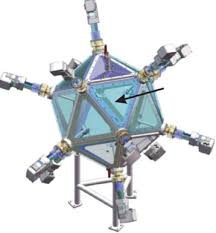
\includegraphics[clip,trim=0 0 0 30,height = 23mm]{LEM.png}\\
	\vspace{-7pt}
	{\hspace{2pt} {\tiny LEM: Zimmerman et al, RSI, 2010}}	
\end{textblock*}
%
\begin{textblock*}{35mm}[0,0](86mm,-4mm)
	\flushleft
	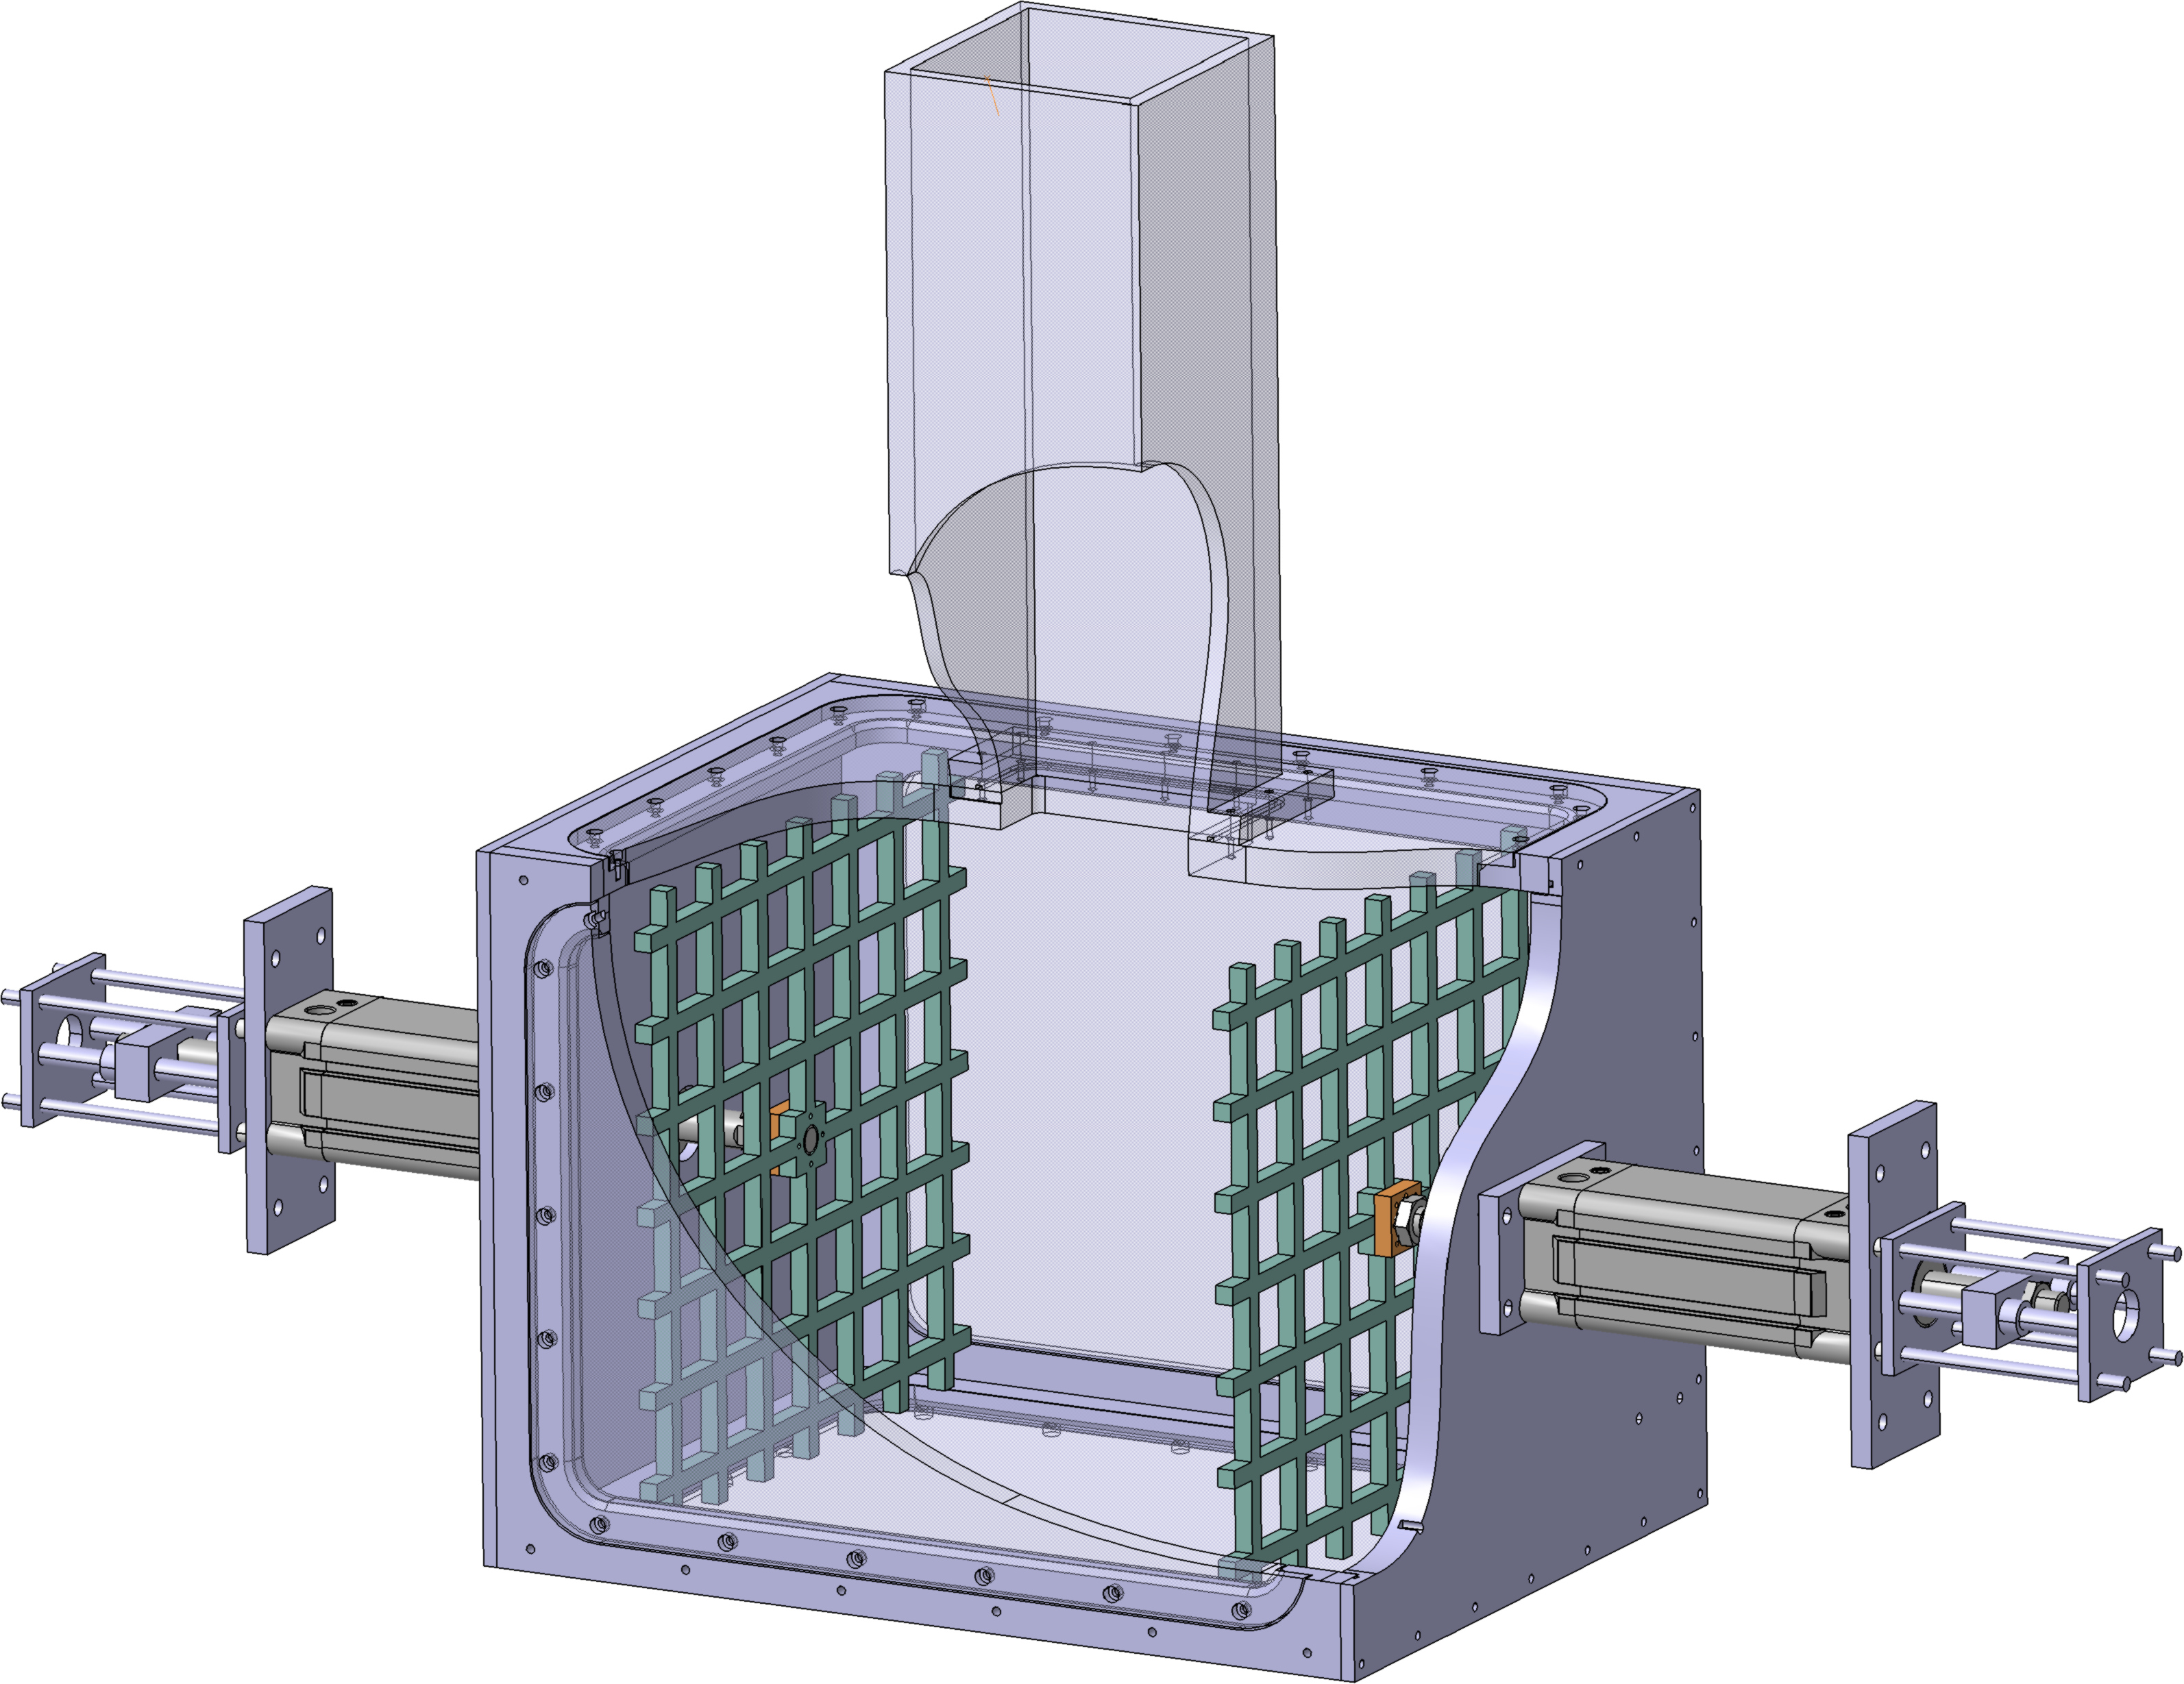
\includegraphics[clip,trim=0 0 0 30,height = 23mm]{Tigrou_isometric_cut2.png}\\
	\vspace{-7pt}
	{\hspace{10pt} {\tiny Oscillating grids: ENSTA}}	
\end{textblock*}
%
\begin{textblock*}{50mm}[0,0](55mm,60mm)
	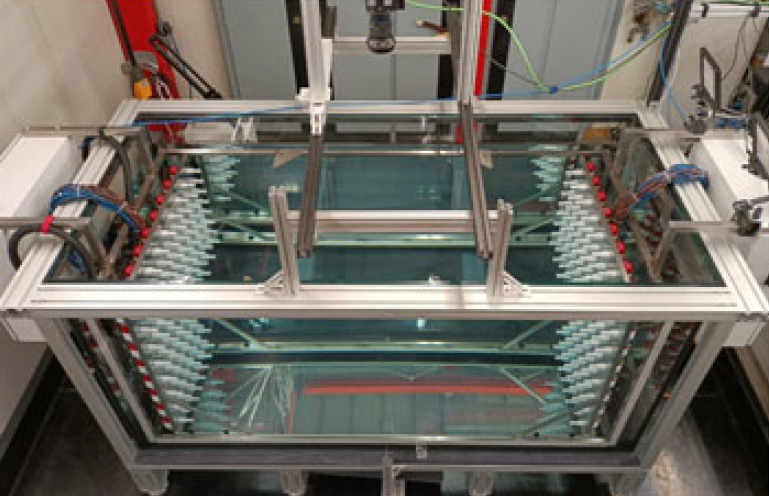
\includegraphics[height = 21mm]{jet_array.png}\\
	\vspace{-6pt}
	{\tiny Jet arrays: Coletti group, Zurich}	
\end{textblock*}

}